\chapter{图与连接结构}
\label{chap:graph-objects}
\label{chap:graph-paths}

城市之间修了哪些道路，一项工程里哪项任务必须等另一项完成，这类信息都由“有限个对象”和“对象之间的直接连接”组成。我们关心的往往不是某一条连接本身，而是由连接串起来的整体：从一座城市能否开车到达另一座，拆掉一座桥以后交通网会不会断成两片，一组任务能否排出不违反依赖的先后次序。回答这些问题之前，先要说清楚记录了什么、没有记录什么。

本章用第~\ref{chap:sets-relations-maps}章的集合、关系与映射建立图这一对象，并回答四个问题：图记录了哪些连接，沿连接能走到哪里，怎样把图交给计算机，什么时候两张图只是换了名字的同一结构。第~\ref{sec:graph-basic-concepts}节定义顶点、边、方向、边权和子图，区分抽象连接与纸上的画法。第~\ref{sec:graph-adjacency-paths}节把一步邻接延长为多步的行走和路径，建立环、有向无环图与可达关系。第~\ref{sec:graph-connectivity-separation}节把可达关系提升为顶点集的划分，并研究删除顶点或边怎样切断连接。第~\ref{sec:graph-trees-forests}节研究有连接而无环的结构，证明树中路径唯一、$n$个顶点的树恰有$n-1$条边。

后两节转向记录与比较。第~\ref{sec:graph-representations}节比较边列表、邻接表、邻接矩阵和关联矩阵，说明各自支持哪种访问、代价随规模怎样增长，并由矩阵乘法推出邻接矩阵的幂计数行走。第~\ref{sec:graph-isomorphism}节用保持邻接的双射刻画同构，再用第三部分的置换矩阵写出重编号。全章用同一张四个顶点、五条边的小图作贯穿例子。

本章只建立定义、基本性质和判定标准。怎样用遍历实际求出连通分量、生成树和拓扑次序是第~\ref{chap:graph-traversal}章的任务；带权路径的最短成本和最小生成树属于第~\ref{chap:graph-optimization}章；沿边计算顶点数值差异的拉普拉斯留到第~\ref{chap:graph-spectral}章。

\section{图的基本概念}
\label{sec:graph-basic-concepts}

一张道路网只需回答“哪些城市之间有一条直达道路”，一份任务清单只需回答“哪项任务直接依赖哪项任务”。两者的共同之处是：对象有限，信息集中在成对对象之间的直接连接上。本节先把这种信息写成图，再分别说明方向、数值和属性给连接添加了什么，最后讨论从一张图中取出一部分时保留了什么。

\subsection{图的定义}
\label{sec:graph-conn-definition}

把每个对象记为一个顶点，把每一对有直接连接的对象记为一条边，就得到一张图。这里先考虑没有方向的连接，例如可以双向通行的道路。

\begin{definition}[图]
\label{def:graph-conn-graph}
设$V$是有限集合，$E$是由$V$中两个不同元素组成的无序对$\{i,j\}$的集合，称$\mathcal G=(V,E)$为一个（无向）\term{图}（graph）。$V$中的元素称为\term{顶点}（vertex），$E$中的元素称为\term{边}（edge）。若$\{i,j\}\in E$，称$i,j$是这条边的两个端点。
\end{definition}

记$n=|V|$为顶点数，$m=|E|$为边数。全章使用同一个例子：
\begin{equation}
V=\{1,2,3,4\},\qquad
E=\bigl\{\{1,2\},\{1,3\},\{2,3\},\{2,4\},\{3,4\}\bigr\},
\label{eq:graph-conn-running-graph}
\end{equation}
它有$n=4$个顶点、$m=5$条边，可以看成两个三角形$\{1,2,3\}$与$\{2,3,4\}$共用边$\{2,3\}$。四个顶点之间最多有$\binom42=6$条边，这里只缺$\{1,4\}$。

\paragraph{图与画法}
图只由集合$V$和$E$确定，纸上的画法不属于图。图~\ref{fig:graph-conn-running-drawings}把同一张图画了三次：顶点的位置不同，线段的长短和弯曲不同，(c)中两条边还在画面上交叉，但三幅图的顶点集和边集完全相同，因此是同一张图。交叉点不是顶点，线段长度也不是边的长度；如果问题需要长度、坐标或其他数值，必须另外指定，见第~\ref{sec:graph-conn-weights}小节。

\begin{figure}[!htb]
  \centering
  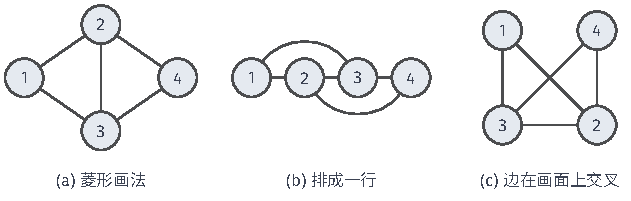
\includegraphics[width=106.765mm]{figures/01-basic-mathematics/04-graphs/tikz/c1-running-graph-drawings/figure.pdf}
  \caption{贯穿全章的四点五边图\eqref{eq:graph-conn-running-graph}的三种画法。顶点位置、线段形状和交叉情况都不同，但边集都是$\{1,2\},\{1,3\},\{2,3\},\{2,4\},\{3,4\}$。(c)中两条对角边在画面上交叉，交叉处不是顶点。}
  \label{fig:graph-conn-running-drawings}
\end{figure}

\paragraph{简单图的约定}
定义~\ref{def:graph-conn-graph}要求边的两个端点不同，并且边集是普通集合，因此排除了两种情形：一个顶点连到自身的\term{自环}（self-loop），以及同一对顶点之间的多条\term{平行边}（parallel edges）。满足这两条限制的图称为\term{简单图}（simple graph），本部分默认讨论有限简单图。若实际问题需要两条平行道路分别记录收费，就要给每条边一个独立身份，不能再把边等同于端点对；这时后面诸如“$n$个顶点最多有$\binom n2$条边”的计数也不再成立。用到这类扩展时会明确指出。

顶点集为空的图只有空边集，它在少数边界情形中出现，例如删除全部顶点后的余图。凡是结论需要至少一个顶点，我们都会写明“非空图”。

\subsection{无向图与有向图}
\label{sec:graph-conn-directions}

道路可以双向通行，“任务$i$完成后才能开始任务$j$”却有先后。无序对$\{i,j\}$不区分两个端点的次序，不能记录后一种信息，因此需要有序对。

\begin{definition}[有向图]
\label{def:graph-conn-digraph}
设$V$是有限集合，$E\subseteq\{(i,j)\in V\times V:i\neq j\}$，称$\mathcal G=(V,E)$为\term{有向图}（directed graph）。有序对$(i,j)\in E$称为从$i$到$j$的\term{弧}（arc），也记作$i\to j$；$i$是它的起点，$j$是它的终点。
\end{definition}

为了区分，以无序对为边的图也称\term{无向图}（undirected graph）。有向图的弧集仍记作$E$，弧数仍记作$m$；需要强调时再说“边或弧”。弧$i\to j$只允许从$i$一步到达$j$，并不包含反向的$j\to i$。

\paragraph{一条无向边不等于两条反向弧}
图~\ref{fig:graph-conn-direction-orientation}(a)(b)对照了无向边$\{u,v\}$与一对反向弧$(u,v),(v,u)$。两者都允许在$u,v$之间来回，但建模含义不同：无向边是一条连接，删除它就同时失去两个方向；两条弧则是两个独立对象，可以只删除其中一条，也可以分别附上不同的数值，例如上坡与下坡的不同用时。把无向图改写成有向图时，可以用一对反向弧代替每条边，但要记住这一步改变了“边”的个数和身份。

\paragraph{方向改变可达的范围}
图~\ref{fig:graph-conn-direction-orientation}(c)--(e)给同一条三点连接1—2—3赋予不同方向。无向时三个顶点两两可以互相到达；定向为$1\to2\to3$后，从$1$可以经$2$到达$3$，从$3$却哪里也去不了；定向为$1\to2\leftarrow3$后，$1$和$3$都只能到达$2$，彼此不能到达。可见方向不只是标注，它直接决定哪些顶点序列允许通行。

\begin{figure}[!htb]
  \centering
  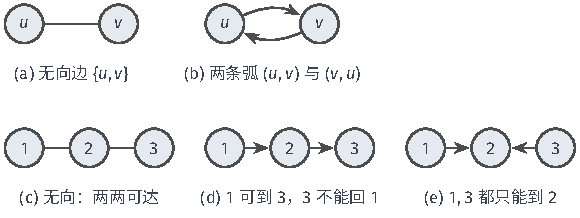
\includegraphics[width=98.189mm]{figures/01-basic-mathematics/04-graphs/tikz/c1-direction-orientation/figure.pdf}
  \caption{方向给连接附加的信息。上排：一条无向边与一对反向弧都允许在$u,v$之间往返，但后者的两条弧可以分别删除或另附数值。下排：同一条三点连接的无向形式(c)与两种定向(d)(e)，箭头决定了从哪个顶点能走到哪个顶点。}
  \label{fig:graph-conn-direction-orientation}
\end{figure}

\paragraph{底层无向图}
忽略有向图每条弧的方向，把$(i,j)$与$(j,i)$都换成无序对$\{i,j\}$（两者同时出现时只留一条边），得到的无向图称为原图的\term{底层无向图}（underlying undirected graph）。图~\ref{fig:graph-conn-direction-orientation}中(d)(e)的底层无向图都是(c)。这一步丢掉了依赖的先后：(c)中$3$能到达$1$，(d)中却不能，所以不能根据底层无向图的连接情况断言原有向图可以双向到达。第~\ref{sec:graph-connectivity-separation}节的弱连通正是建立在底层无向图上的概念，那里会再次比较两者。

\subsection{边权与属性}
\label{sec:graph-conn-weights}

图只说明哪些顶点直接相连。许多问题还需要每条连接上的一个数：道路有多长，管道每秒最多输送多少，两个样本有多相似。

\paragraph{边权的三种常见语义}
给每条边$\{i,j\}$（或弧$(i,j)$）附加一个实数，称为\term{边权}（edge weight）。图~\ref{fig:graph-conn-weight-semantics}在同一个边集上附加了同一组数，却给出三种读法。读作长度$\ell_{i,j}$时，数值沿路线逐条相加，路线$1,2,4$的总长是$2+1=3$，越小越好；读作容量$c_{i,j}$时，数值是通过这条边的流量上限，边$\{1,3\}$上至多通过$1$个单位，容量不沿路线相加；读作相似度$w_{i,j}$时，权重越大，后续计算越强地要求两端取值接近。同一个数字$1$在三种问题里参与的运算完全不同，所以拿到一张带权图时，要先问清权重的用途，再选择方法。

\begin{figure}[!htb]
  \centering
  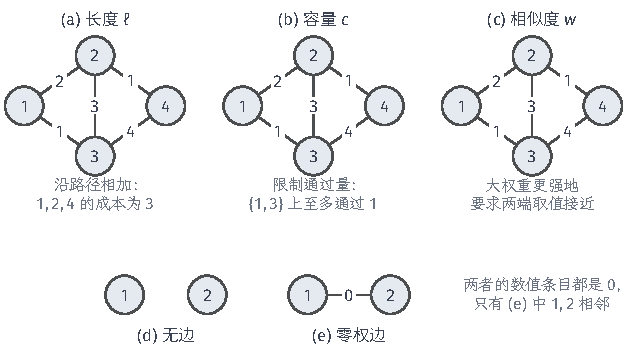
\includegraphics[width=106.768mm]{figures/01-basic-mathematics/04-graphs/tikz/c1-weight-semantics/figure.pdf}
  \caption{同一边集上的同一组边权在三种问题中的读法。(a)长度沿路线相加，路线$1,2,4$的总长为$3$；(b)容量限制单条边的通过量；(c)相似度越大，越要求两端取值接近。下排对照无边(d)与零权边(e)：二者在数值上都记为$0$，但只有(e)中顶点$1,2$相邻。}
  \label{fig:graph-conn-weight-semantics}
\end{figure}

\paragraph{无边与零权边}
边权为$0$并不等于没有边。零长度的道路表示免费通行，零容量的管道不能输送正流量，零相似度在加权求和中不贡献数值；但在这三种情形中，结构上的边都还在。图~\ref{fig:graph-conn-weight-semantics}(d)(e)中，两个顶点之间有没有边由边集决定，与边权是否为零无关：“能否一步到达”查边集，“沿边累计多少”查边权。第~\ref{sec:graph-representations}节用矩阵记录图时，这一区别会变成一个具体的存储问题。

边权能否为负，也由问题决定。负长度可以表示途经某处得到补贴，它会让最短路问题出现新的困难；谱方法则要求相似度非负。这些条件分别在第~\ref{chap:graph-optimization}章和第~\ref{chap:graph-spectral}章建立，本章不预设边权的符号。

\paragraph{顶点属性与边属性}
除了一个实数，边上还可以记录类别、时间等其他数据，顶点上也可以记录人口、坐标等数据，分别称为边属性和顶点属性。顶点的名称$1,2,3,4$只用来区分顶点，本身不是属性：第~\ref{sec:graph-isomorphism}节比较两张图时会看到，换一套名称不改变图的结构，而属性是否必须保持则要由问题声明。

\subsection{子图与诱导子图}
\label{sec:graph-conn-subgraphs}

研究道路网时，常常只关心其中一部分城市，或者想知道封闭几条道路后还剩什么。这两种操作都从原图取出一部分，但保留的东西不同。

\paragraph{子图}
若$V'\subseteq V$，$E'\subseteq E$，并且$E'$中每条边的两个端点都在$V'$中，称$\mathcal G'=(V',E')$是$\mathcal G$的\term{子图}（subgraph）。最后一条要求保证$\mathcal G'$本身仍是一张图，不会出现端点被删掉的边。两种基本操作都产生子图：删除一条边$e$只去掉这条边，顶点全部保留，记作$\mathcal G-e$；删除一个顶点集$S$则去掉$S$中的顶点以及所有至少有一个端点在$S$中的边，记作$\mathcal G-S$。

在图~\ref{fig:graph-conn-subgraph-induced}中，(b)(c)两个子图保留同一组顶点$\{1,2,3\}$，边集却不同：(b)保留三条边，(c)只保留$\{1,2\}$与$\{2,3\}$。所以只给出顶点集合，还不能确定一个一般子图；(d)则是只删除边$\{2,3\}$、保留全部顶点的子图。

\begin{figure}[!htb]
  \centering
  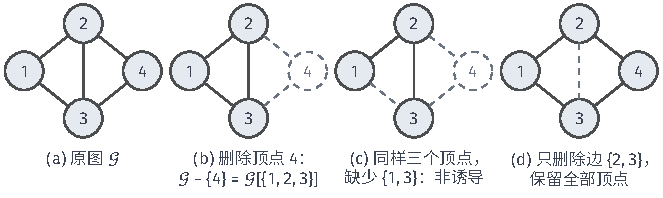
\includegraphics[width=112.000mm]{figures/01-basic-mathematics/04-graphs/tikz/c1-subgraph-induced/figure.pdf}
  \caption{贯穿图的几种子图，灰色虚线表示被删除的顶点或边。(b)删除顶点$4$及其两条边，恰好得到顶点集$\{1,2,3\}$上的诱导子图；(c)保留同样三个顶点，却漏掉了原图中的边$\{1,3\}$，是子图但不是诱导子图；(d)只删除一条边，顶点全部保留。}
  \label{fig:graph-conn-subgraph-induced}
\end{figure}

\paragraph{诱导子图}
只研究一部分顶点时，通常不希望悄悄改变这些顶点之间的关系。为此固定顶点子集，把原图中两端都在其中的边全部保留下来。

\begin{definition}[诱导子图]
\label{def:graph-conn-induced-subgraph}
设$S\subseteq V$。以$S$为顶点集、以$\{\{i,j\}\in E:i,j\in S\}$为边集的子图，称为$\mathcal G$在$S$上的\term{诱导子图}（induced subgraph），记作$\mathcal G[S]$。有向图的诱导子图保留两端都在$S$中的全部弧。
\end{definition}

诱导子图由顶点集唯一确定。图~\ref{fig:graph-conn-subgraph-induced}(b)是$\mathcal G[\{1,2,3\}]$，它必须保留三角形的三条边；(c)虽然顶点相同，但缺少$\{1,3\}$，不是诱导子图。删除顶点与取诱导子图互为补充：$\mathcal G-S=\mathcal G[V\setminus S]$。后面讨论删除一组顶点能否切断连接（第~\ref{sec:graph-connectivity-separation}节），以及第~\ref{chap:graph-traversal}章把图按分隔集分块时，用到的都是这一记号。

\section{邻接与路径}
\label{sec:graph-adjacency-paths}

贯穿图\eqref{eq:graph-conn-running-graph}中顶点$1$和$4$之间没有边，却可以先到$2$或$3$，再到$4$。“一步能到谁”由边集直接读出；“若干步能到谁”则要把边首尾相接。本节先描述一个顶点的直接邻居，再定义多步的行走和路径，区分无向环与有向环，最后建立可达关系。边上若有长度，怎样比较不同路线的总成本是第~\ref{sec:graph-shortest-paths}节的问题，这里只讨论哪些顶点序列允许通行。

\subsection{邻接、邻域与度}
\label{sec:graph-conn-neighborhoods}

在无向图中，若$\{i,j\}\in E$，称$i$与$j$\term{邻接}（adjacent），互为邻居。顶点$i$的全部邻居组成它的\term{邻域}（neighborhood）
\[
N(i)=\{j\in V:\{i,j\}\in E\},
\]
邻居的个数$d_i=|N(i)|$称为$i$的\term{度}（degree）。贯穿图中$N(1)=\{2,3\}$，$N(2)=\{1,3,4\}$，四个顶点的度依次为$2,3,3,2$。度只数直接邻居；$1$经过两步可以到达$4$，但$4$不计入$N(1)$。

\paragraph{有向图的两种邻域}
在有向图中，一条弧$i\to j$对两个端点的意义不同：对$i$来说$j$是下一步可以到达的顶点，对$j$来说$i$是能一步到达它的顶点。因此要分别定义出邻域与入邻域：
\[
N^+(i)=\{j:(i,j)\in E\},\qquad
N^-(i)=\{j:(j,i)\in E\}.
\]
二者的大小$d_i^+=|N^+(i)|$与$d_i^-=|N^-(i)|$分别称为\term{出度}（out-degree）与\term{入度}（in-degree）。以图~\ref{fig:graph-conn-direction-orientation}(e)的$1\to2\leftarrow3$为例，$N^-(2)=\{1,3\}$，$N^+(2)=\varnothing$：两个顶点能一步到达$2$，从$2$出发却一步也走不了。报告“$2$的邻居”时若不说明方向，就可能把入邻居误当成下一步可以到达的顶点。

\paragraph{度数和与边数}
把每个顶点的度加起来，会得到一个只与边数有关的量。考虑所有“顶点—边”配对$(i,e)$，其中$i$是边$e$的端点。按顶点分组，顶点$i$出现在$d_i$个配对中；按边分组，每条边恰有两个端点，出现在两个配对中。两种分组数的是同一批配对，所以
\begin{equation}
\sum_{i\in V}d_i=2m.
\label{eq:graph-conn-handshake}
\end{equation}
贯穿图中$2+3+3+2=10=2\times5$。由此还可知，度为奇数的顶点个数必是偶数，否则左边为奇数。在有向图中，每条弧恰好贡献一个出度和一个入度，同样的分组给出
\[
\sum_{i\in V}d_i^+=\sum_{i\in V}d_i^-=m;
\]
例如图~\ref{fig:graph-conn-direction-orientation}(d)的$1\to2\to3$中，出度为$1,1,0$，入度为$0,1,1$，两组之和都是弧数$2$。这里的度只数结构上的边，不涉及边权；把邻边权重累加起来的加权度在第~\ref{sec:graph-vertex-edge-functions}节另行定义。

\subsection{行走、路径与环}
\label{sec:graph-conn-walks-paths}

把相邻的边首尾相接，就得到一串顶点。是否允许重复经过同一个顶点，会得到用途不同的对象：反复传播、来回巡视的过程允许重复，一条实际路线通常不允许。

\begin{definition}[行走与路径]
\label{def:graph-conn-walk-path}
设$\mathcal G=(V,E)$是无向图。顶点序列$(v_0,\ldots,v_k)$若对每个$r=1,\ldots,k$都有$\{v_{r-1},v_r\}\in E$，就称为从$v_0$到$v_k$的一条\term{行走}（walk），$k$称为它的长度，即经过的边数。若行走中的顶点两两不同，就称为一条简单\term{路径}（path）。
\end{definition}

行走允许重复经过顶点和边；单个顶点$(v_0)$是长度为零的行走，也是长度为零的路径。本部分不加修饰的“路径”都指简单路径。图~\ref{fig:graph-conn-walk-path-cycle}(a)的$(1,2,3,1,2)$是长度为$4$的行走，它两次经过边$\{1,2\}$；(b)的$(1,2,4)$是长度为$2$的路径。

\begin{figure}[!htb]
  \centering
  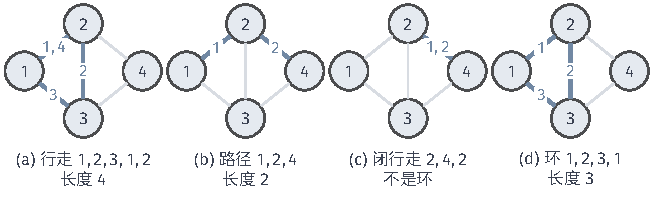
\includegraphics[width=110.688mm]{figures/01-basic-mathematics/04-graphs/tikz/c1-walk-path-cycle/figure.pdf}
  \caption{贯穿图上的四种顶点序列。蓝色粗线是经过的边，边旁数字是经过该边的步序，浅灰色是未经过的边。(a)行走可以重复经过边$\{1,2\}$；(b)路径不重复顶点；(c)沿一条边去而复返得到闭行走，但它不是环；(d)绕三角形一周的环除首尾外不重复顶点。}
  \label{fig:graph-conn-walk-path-cycle}
\end{figure}

\paragraph{闭行走与环}
首尾相同（$v_0=v_k$）的行走称为\term{闭行走}（closed walk）。闭合并不意味着绕成了一圈：图~\ref{fig:graph-conn-walk-path-cycle}(c)的$(2,4,2)$沿边$\{2,4\}$去而复返，是长度为$2$的闭行走，却没有围出任何区域。为了排除这种情形，把长度$k\geq3$、且$v_0,v_1,\ldots,v_{k-1}$两两不同的闭行走称为\term{环}（cycle）。长度下限来自简单图的约定：长度为$1$的闭行走需要自环，长度为$2$的闭行走$(v_0,v_1,v_0)$只能沿同一条边往返。图~\ref{fig:graph-conn-walk-path-cycle}(d)的$(1,2,3,1)$是长度为$3$的环。

同一个环可以从不同顶点出发、沿两个方向书写，例如$(1,2,3,1)$、$(2,3,1,2)$和$(1,3,2,1)$经过的是同一组边。计数环或比较两个环时，我们把经过同一组边的序列看成同一个环。

\subsection{有向路径与有向无环图}
\label{sec:graph-conn-dag}

任务依赖要求每一步都顺着箭头走：从任务$i$出发，只能走到依赖$i$的任务。把定义~\ref{def:graph-conn-walk-path}中的条件$\{v_{r-1},v_r\}\in E$换成$(v_{r-1},v_r)\in E$，就得到有向行走与\term{有向路径}（directed path）；长度、闭合与顶点不重复的含义不变。

\paragraph{有向环}
除首尾外顶点两两不同、长度至少为$1$的有向闭行走称为\term{有向环}（directed cycle）。由于排除了自环，有向环的长度至少为$2$；与无向情形不同，长度为$2$的有向环是允许的。图~\ref{fig:graph-conn-directed-cycle-dag}(a)中两条反向弧$i\to j$和$j\to i$是两个不同的对象，$(i,j,i)$依次经过它们，构成一个有向环；而无向图中的$(2,4,2)$两次经过的是同一条边。图~\ref{fig:graph-conn-directed-cycle-dag}(b)的$(1,2,3,1)$每一步都顺着箭头，是长度为$3$的有向环。

\begin{figure}[!htb]
  \centering
  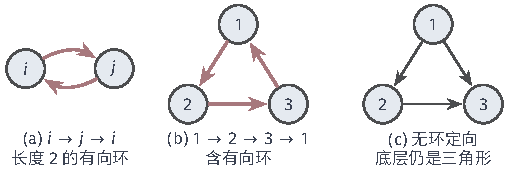
\includegraphics[width=85.937mm]{figures/01-basic-mathematics/04-graphs/tikz/c1-directed-cycle-dag/figure.pdf}
  \caption{有向环与有向无环图。红色弧组成有向环。(a)两条反向弧构成长度为$2$的有向环；(b)三角形的循环定向含有向环；(c)同一个三角形的另一种定向不含有向环，是有向无环图，尽管它的底层无向图是一个环。}
  \label{fig:graph-conn-directed-cycle-dag}
\end{figure}

\paragraph{有向无环图}
如果任务之间的依赖形成有向环，例如$1$等$2$、$2$等$3$、$3$又等$1$，这组任务就无法按任何次序全部完成。不含有向环的依赖才可能排出顺序。

\begin{definition}[有向无环图]
\label{def:graph-conn-dag}
不含有向环的有向图称为\term{有向无环图}（directed acyclic graph，DAG）。
\end{definition}

“无环”只针对有向环。图~\ref{fig:graph-conn-directed-cycle-dag}(c)的弧为$1\to2$、$1\to3$、$2\to3$，逐个检查长度为$2$和$3$的闭合序列，没有一个能每步都顺着箭头：例如$(1,2,3,1)$的最后一步需要弧$3\to1$，而图中只有$1\to3$。所以它是DAG，但去掉箭头后得到一个三角形，底层无向图是有环的。第~\ref{sec:graph-topological-order}节的拓扑排序要求的正是有向无环，不能换成“底层无向图无环”这个更强的条件。

\subsection{可达性}
\label{sec:graph-conn-reachability}

前面的定义描述的是具体的顶点序列。很多问题只关心“能不能到”，而不关心怎么到。

\paragraph{可达关系}
若存在从$i$到$j$的行走，称$j$从$i$\term{可达}（reachable）；有向图中要求有向行走。行走允许重复顶点，使用起来比路径方便：从$i$到$j$的行走接上从$j$到$k$的行走，仍是一条行走，而两条路径首尾相接后可能重复经过顶点。下面的引理说明，判断可达时用行走还是路径并没有区别。

\begin{lemma}[行走中含有路径]
\label{lem:graph-conn-walk-contains-path}
在无向图或有向图中，若存在从$i$到$j$的行走，则存在从$i$到$j$的路径，并且它的顶点和边都取自这条行走。
\end{lemma}

\begin{proof}
在从$i$到$j$、顶点和边都取自原行走的所有行走中，取长度最短的一条$(v_0,\ldots,v_k)$。若它不是路径，则有$s<t$使$v_s=v_t$。删去中间段$v_{s+1},\ldots,v_t$，得到$(v_0,\ldots,v_s,v_{t+1},\ldots,v_k)$：原来从$v_t$出发的那一步现在从$v_s=v_t$出发，因此每一步仍沿原有的边或弧，而长度减少了$t-s>0$，与长度最短矛盾。所以最短的那条行走就是路径。
\end{proof}

由定义和引理，可达关系有以下性质。零长度行走使每个顶点从自身可达，即自反性；行走首尾相接说明传递性；在无向图中把行走倒过来走仍是行走，所以还有对称性。因此无向图上的可达关系是第~\ref{sec:prelim-equivalence-relations}节意义下的等价关系，下一节将据此划分连通分量。

\paragraph{有向图中可达不对称}
有向图中倒过来走需要反向弧，对称性一般不成立。在图~\ref{fig:graph-conn-direction-orientation}(d)的单向链$1\to2\to3$中，$3$从$1$可达，$1$却不从$3$可达。为了描述这种单向的关系，把一步关系与多步关系分别命名：$N^-(j)$中的顶点称为$j$的直接\term{前驱}（predecessor），$N^+(j)$中的顶点称为直接\term{后继}（successor）；能经过一条或多条弧到达$j$的其他顶点称为$j$的\term{祖先}（ancestor），从$j$出发经过一条或多条弧能到达的其他顶点称为$j$的\term{后代}（descendant）。本部分约定祖先与后代都不含$j$自身。

在单向链中，$3$的直接前驱只有$2$，祖先则是$\{1,2\}$；$1$的后代是$\{2,3\}$，$3$没有后代。有向环上的两个不同顶点可以互为祖先，例如图~\ref{fig:graph-conn-directed-cycle-dag}(b)中的$1$和$2$；在DAG中这不可能发生。若$i\neq j$互为祖先，把$i$到$j$与$j$到$i$的两条有向路径拼起来，得到一条长度至少为$2$的有向闭行走$(v_0,\ldots,v_k)$，其中$v_0=v_k$。在所有满足$s<t$、$v_s=v_t$的位置对中取$t-s$最小的一对，则$(v_s,\ldots,v_t)$除首尾外不重复顶点；它的长度不能为$1$（没有自环），所以是一个有向环，与DAG的定义矛盾。可达的不对称性使有向图的“连通”需要两种不同的定义，这是下一节的内容。

\section{连通与分隔}
\label{sec:graph-connectivity-separation}

上一节的可达关系一次只回答两个顶点之间的问题。道路网规划还需要整体的回答：全部城市分成几片互相到达的区域，封闭哪些路口或道路会把区域切开。本节先用可达关系把顶点集划分为连通分量，再对有向图区分强、弱两种连通，最后研究删除顶点或边怎样改变连接。这里只讨论结构上的路径是否存在，不涉及概率中的条件独立；后者有自己的分离判据，留到后续关于推断的部分。

\subsection{无向图的连通分量}
\label{sec:graph-conn-components}

在无向图中，可达关系是等价关系（第~\ref{sec:graph-conn-reachability}小节）。由定理~\ref{thm:sets-equivalence-partition}，它的等价类构成顶点集的一个划分。

\begin{definition}[连通分量]
\label{def:graph-conn-component}
无向图$\mathcal G=(V,E)$中可达关系的每个等价类$C\subseteq V$称为$\mathcal G$的一个\term{连通分量}（connected component）；有时也把诱导子图$\mathcal G[C]$称为连通分量。若$\mathcal G$非空且恰有一个连通分量，即任意两个顶点之间都有路径，就称$\mathcal G$是\term{连通}（connected）的。
\end{definition}

这个划分有三条直接的性质。第一，同一分量中任意两点可达，而且连接它们的路径不会离开该分量，因为路径上的每个顶点都与起点可达；所以$\mathcal G[C]$本身是连通图。第二，不同分量之间没有边：若$i\in C$、$j\in C'$之间有边，则$j$从$i$可达，二者应属同一分量。第三，划分由图唯一确定，因为等价类只取决于可达关系本身，与我们从哪个顶点开始寻找无关。

图~\ref{fig:graph-conn-components}(a)是三角形$\{1,2,3\}$加上孤立顶点$4$。$4$没有邻居，只与自身可达，单独构成一个分量，所以这张图有两个分量$\{1,2,3\}$与$\{4\}$，不连通。对顶点集为空的图，可达关系没有等价类，分量数为$0$；按定义它不算连通图。凡是用“恰有一个分量”判断连通性的论证，都需要先排除这个边界情形。

\begin{figure}[!htb]
  \centering
  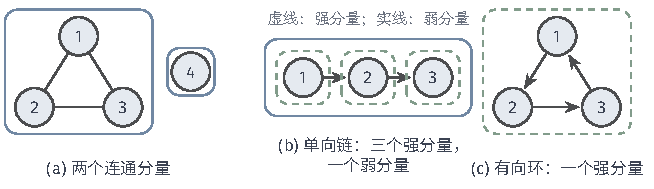
\includegraphics[width=110.808mm]{figures/01-basic-mathematics/04-graphs/tikz/c1-components/figure.pdf}
  \caption{连通分量。蓝色实线框是无向图或底层无向图的连通分量，绿色虚线框是强连通分量。(a)孤立点自成一个分量；(b)单向链$1\to2\to3$忽略方向后连成一片，但没有两个顶点能互相到达，每个顶点自成一个强分量；(c)有向环上任意两个顶点都能互相到达，三个顶点属于同一个强分量。}
  \label{fig:graph-conn-components}
\end{figure}

\paragraph{删除边与替代路径}
连通性取决于是否还有替代路径，而不只取决于边的数目。在贯穿图中删除边$\{2,3\}$，$2$与$3$仍可经$1$或$4$相连，图依然连通；在图~\ref{fig:graph-conn-cut-bridge}(a)中删除连接两个三角形的边$\{3,4\}$，两侧之间就再没有路径，图分成两个分量。两次都只删除了一条边，结果不同的原因是前者的边位于环上，环的另一侧提供了替代路径。第~\ref{sec:graph-conn-separators}小节会把这一观察写成桥的判别条件。

\subsection{强连通与弱连通}
\label{sec:graph-conn-strong-weak}

有向图中可达不对称，“$j$从$i$可达”不能像无向图那样直接用来划分顶点。有两种自然的修补：要求双向都可达，或者干脆忽略方向。

\paragraph{强连通分量}
若$j$从$i$可达且$i$从$j$可达，称$i,j$相互可达。相互可达关系是自反的（零长度行走）、对称的（定义本身对$i,j$对称）、传递的（两个方向分别把行走首尾相接），因此是等价关系。它的等价类称为\term{强连通分量}（strongly connected component）；若有向图非空且只有一个强连通分量，即任意有序顶点对$(i,j)$之间都有从$i$到$j$的有向路径，就称它\term{强连通}（strongly connected）。

图~\ref{fig:graph-conn-components}(b)的单向链中，$1$能到$3$而$3$不能到$1$，任何两个不同顶点都不相互可达，所以三个顶点各自构成一个强分量。(c)的有向环中，从任一顶点出发沿环走一段就能到达其他任一顶点，三个顶点同属一个强分量，图是强连通的。可见强分量把“绕得回来”的顶点归在一起；把单向可达的顶点合进同一个强分量是错误的。

\paragraph{弱连通分量}
忽略方向后，用底层无向图（第~\ref{sec:graph-conn-directions}小节）的连通分量来划分顶点，所得的分量称为原图的\term{弱连通分量}（weakly connected component）；底层无向图连通时，称原有向图\term{弱连通}（weakly connected）。图~\ref{fig:graph-conn-components}(b)的单向链去掉箭头后是一条路径，只有一个弱分量。

两种分量的关系是单向的。每条有向路径去掉箭头后都是底层无向图中的路径，所以相互可达的两个顶点必在同一个弱分量中：每个强分量都包含在某个弱分量之内，强连通蕴含弱连通。反过来不成立，单向链弱连通但不强连通，其中$3$到不了$1$。所以弱连通只说明忽略方向后连成一片，不保证任何两个顶点能双向到达。怎样在线性时间内求出全部强分量，是第~\ref{sec:graph-connectivity-computation}节的内容。

\subsection{分隔集、割点与桥}
\label{sec:graph-conn-separators}

连通分量描述的是现状；规划者还关心脆弱性：封闭哪些路口能把两个区域隔开，哪个单独的路口或哪条单独的道路一旦失效就会让网络断开。

\paragraph{分隔集}
要把两组顶点隔开，就要删除一些别的顶点，使两组之间不再有路径。被删除的顶点不能属于要隔开的两组本身。

\begin{definition}[分隔]
\label{def:graph-conn-separation}
设$A,B,S\subseteq V$两两不相交。若在$\mathcal G-S$中不存在从$A$中顶点到$B$中顶点的路径，就称$S$\term{分隔}（separate）$A$与$B$，称$S$为$A$与$B$之间的一个\term{分隔集}（separator）。
\end{definition}

等价地，$\mathcal G$中从$A$到$B$的每条路径都至少经过$S$中的一个顶点：若某条路径避开了$S$，它在$\mathcal G-S$中仍然存在。这个等价说法提醒我们，验证一个候选集要检查全部路径，找到一条被阻断的路径并不够。

在图~\ref{fig:graph-conn-separator-sets}中取$A=\{1\}$、$B=\{4\}$。候选集$S=\{2\}$阻断了路径$(1,2,4)$，但$\mathcal G-\{2\}$中仍有路径$(1,3,4)$，所以$\{2\}$不分隔$1$与$4$；删除$S=\{2,3\}$后，$1$的邻居全部被删除，$1$与$4$之间不再有路径，$\{2,3\}$才是分隔集。若$A$与$B$在原图中已经位于不同分量，空集就分隔它们，因为不删除任何顶点时本来就没有路径。

\begin{figure}[!htb]
  \centering
  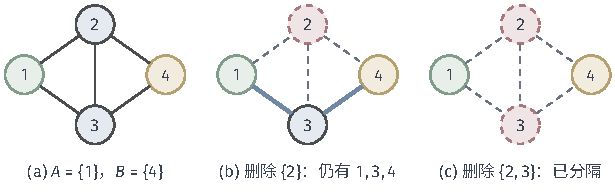
\includegraphics[width=104.186mm]{figures/01-basic-mathematics/04-graphs/tikz/c1-separator-sets/figure.pdf}
  \caption{在贯穿图中检验分隔集，$A=\{1\}$为绿色，$B=\{4\}$为黄色，被删除的候选集$S$为红色虚线顶点。(b)删除$\{2\}$后蓝色路径$(1,3,4)$仍然存在，$\{2\}$不是分隔集；(c)删除$\{2,3\}$后从$1$到$4$没有路径，$\{2,3\}$分隔$\{1\}$与$\{4\}$。}
  \label{fig:graph-conn-separator-sets}
\end{figure}

不指定$A,B$时，也可以只问删除一组顶点后图是否断开。对连通图$\mathcal G$，若$\mathcal G-S$不连通，则$S$分隔$\mathcal G-S$中任意两个不同分量的顶点集。例如贯穿图删除$\{2,3\}$后余下$\{1\}$与$\{4\}$两个分量。第~\ref{sec:graph-separator-blocks}节将沿这样的分隔集把图分成可以分别处理的块。

\paragraph{割点与桥}
最脆弱的情形是只删除一个顶点或一条边就增加了分量数。删除顶点$v$后$\mathcal G-\{v\}$的分量数大于$\mathcal G$的分量数，称$v$为\term{割点}（cut vertex）；删除边$e$后$\mathcal G-e$的分量数大于$\mathcal G$的分量数，称$e$为\term{桥}（bridge）。

图~\ref{fig:graph-conn-cut-bridge}(a)由两个三角形和连接它们的边$\{3,4\}$组成。删除$3$后，$\{1,2\}$与$\{4,5,6\}$分开，$4$同理，所以$3,4$是割点；删除边$\{3,4\}$也把两侧分开，它是桥。三角形内部的边都不是桥，三角形顶点$1,2,5,6$也不是割点。(b)的链中，中间顶点$2$是割点，两条边都是桥；(c)的三角形中，删除任意一个顶点或一条边，剩下的部分仍然连通。

\begin{figure}[!htb]
  \centering
  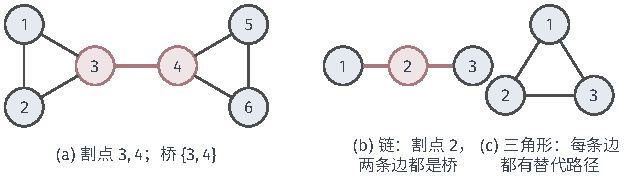
\includegraphics[width=106.765mm]{figures/01-basic-mathematics/04-graphs/tikz/c1-cut-vertex-bridge/figure.pdf}
  \caption{割点与桥，红色顶点为割点，红色粗边为桥。(a)两个三角形由一条边相连，这条边是桥，它的两个端点是割点；(b)链上每条边都是桥，中间顶点是割点，端点$1,3$虽是桥的端点却不是割点；(c)三角形的每条边都位于环上，删除任何一条边或一个顶点都不会断开。}
  \label{fig:graph-conn-cut-bridge}
\end{figure}

\paragraph{为什么边位于环上就不是桥}
设$e=\{i,j\}$。删除$e$只可能拆开$e$所在的那个分量$C$：$C$中任一顶点$x$在原图中有到$i$的路径，若这条路径不经过$e$，删除后它仍连到$i$；若经过$e$，取它第一次到达$i$或$j$之前的部分，删除后$x$仍连到$i$或$j$。所以$\mathcal G-e$中$C$至多分成$i$所在和$j$所在两部分，分量数至多增加$1$。由此得到判别条件：$e$是桥，当且仅当$\mathcal G-e$中没有从$i$到$j$的路径。

若$e$位于某个环上，沿环的另一侧就是$\mathcal G-e$中从$i$到$j$的路径，$e$不是桥。反过来，若$\mathcal G-e$中有从$i$到$j$的路径$P$，它不经过$e$，长度至少为$2$，接上$e$就得到一个环。所以一条边是桥，当且仅当它不在任何环上。这正是图~\ref{fig:graph-conn-cut-bridge}中三角形与链的区别。

\paragraph{顶点分隔与边分隔不同}
删除一个顶点会同时删除它的全部邻边，可能把分量拆成很多块：在一个中心顶点与其余每个顶点各连一条边的星形图中，删除中心顶点后，其余每个顶点都自成一个分量。删除一条边却如上所述至多增加一个分量。此外，桥的端点不一定是割点，例如图~\ref{fig:graph-conn-cut-bridge}(b)的端点$1$；没有桥的图也可能有割点，例如两个三角形共用一个顶点时，共用的顶点是割点，而每条边都在某个三角形上。所以“删点能否断开”与“删边能否断开”需要分别检查。

\section{树与森林}
\label{sec:graph-trees-forests}

上一节看到，边位于环上时删掉它不会断开连接，环提供的是冗余的替代路径。反过来，若要用尽量少的道路把一组城市连起来，就不应保留任何环。本节研究连通而无环的结构：先给出树和森林的定义，再证明树中路径唯一、$n$个顶点的树恰有$n-1$条边，然后在树上选根来组织父子关系，最后从一般连通图中抽取覆盖全部顶点的树。这些结论是第~\ref{chap:graph-traversal}章遍历结果、第~\ref{sec:graph-minimum-spanning-tree}节最小生成树和第~\ref{sec:graph-tree-dp}节树上动态规划的共同基础。

\subsection{树与森林的定义}
\label{sec:graph-conn-tree-definition}

连通保证任意两点之间有路线，无环保证没有多余的路线。同时要求这两点，就得到树。

\begin{definition}[树与森林]
\label{def:graph-conn-tree}
非空、连通且不含环的无向图称为\term{树}（tree）。不含环的无向图称为\term{森林}（forest）。
\end{definition}

森林的每个连通分量都是连通且无环的，因而都是一棵树，“森林”的名称由此而来。不同分量之间没有边，所以森林整体未必连通，只有恰好一个分量的森林才是树。图~\ref{fig:graph-conn-tree-forest}给出几个对照：(a)的链和(b)的星形都是树，树可以有分支，不必排成一条线；(c)的三角形连通但有环，不是树；(d)有三个分量$\{1,2\}$、$\{3,4,5\}$和$\{6\}$，每个都是树，整体是森林而不是树。

\begin{figure}[!htb]
  \centering
  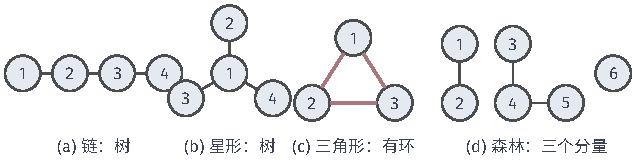
\includegraphics[width=107.685mm]{figures/01-basic-mathematics/04-graphs/tikz/c1-tree-forest/figure.pdf}
  \caption{树、森林与非树的对照。(a)链与(b)星形都是树，后者有分支；(c)三角形连通但含有红色标出的环，不是树；(d)由三个互不相连的树组成的森林，其中孤立顶点$6$是一棵单点树。}
  \label{fig:graph-conn-tree-forest}
\end{figure}

两个边界情形需要单独说明。只有一个顶点、没有边的图是树，称为单点树；图~\ref{fig:graph-conn-tree-forest}(d)中的顶点$6$就是森林里的一棵单点树，所以树中的顶点不必都有邻边。顶点集为空的图不含环，按定义是森林，称为空森林，它有$0$个分量；但树要求非空，所以空图不是树。

\subsection{树的基本性质}
\label{sec:graph-conn-tree-properties}

树的定义由连通和无环两条组成，这两条恰好对应路径的存在与唯一。下面先证明这一点，再用叶顶点数出树的边数。

\paragraph{路径唯一性}
若两点之间有两条不同的路径，它们分开以后终究要在某处会合，分开与会合之间的两段就围成一个环。反过来，环上相邻的两点既有一条边直接相连，又可以沿环的另一侧到达。这两个观察合起来给出下面的等价刻画。

\begin{theorem}[树中路径唯一]
\label{thm:graph-conn-tree-unique-path}
设$\mathcal G$是非空无向图。$\mathcal G$是树，当且仅当任意两个顶点之间恰有一条路径。
\end{theorem}

\begin{proof}
先设$\mathcal G$是树。连通性保证任意两点$u,v$之间至少有一条路径。假设有两条不同的路径$P=(p_0,\ldots,p_a)$与$Q=(q_0,\ldots,q_b)$，$p_0=q_0=u$，$p_a=q_b=v$。一条不能是另一条的真前段，否则较长的那条会两次经过$v$；所以存在最小的$s$使$p_{s+1}\neq q_{s+1}$，记$x=p_s=q_s$，两条路径在$x$处分开。由于$v$同时在两条路径上，可以取$P$在$x$之后第一个也出现在$Q$中$x$之后的顶点$y$。

$P$从$x$到$y$的一段与$Q$从$x$到$y$的一段除端点外没有公共顶点：$P$这一段的中间顶点按$y$的取法不在$Q$中$x$之后的部分，又因为$P$是路径，也不在$P$与$Q$共有的$x$之前的部分。沿$P$从$x$走到$y$，再沿$Q$倒着从$y$走回$x$，就得到一个除首尾外不重复顶点的闭行走。两段不能都只有一条边，否则$p_{s+1}=y=q_{s+1}$；所以它的长度至少为$3$，是一个环，与树无环矛盾。图~\ref{fig:graph-conn-tree-properties}(a)画出了这个构造。

反过来，设任意两点之间恰有一条路径。路径的存在说明$\mathcal G$连通。若$\mathcal G$含环$(c_0,c_1,\ldots,c_{k-1},c_0)$，$k\geq3$，则$(c_0,c_1)$与$(c_0,c_{k-1},c_{k-2},\ldots,c_1)$是从$c_0$到$c_1$的两条不同路径，与唯一性矛盾。所以$\mathcal G$无环，是树。
\end{proof}

由这个定理，删除树的任意一条边$e=\{u,v\}$都会把树断开：$u,v$之间唯一的路径就是$(u,v)$本身，删除$e$后它们之间不再有路径。按第~\ref{sec:graph-conn-separators}小节的论证，树恰好分成$u$所在与$v$所在的两部分，每部分仍连通且无环，是两棵较小的树。换言之，树的每条边都是桥，删去一条边就把树分成两侧。

\begin{figure}[!htb]
  \centering
  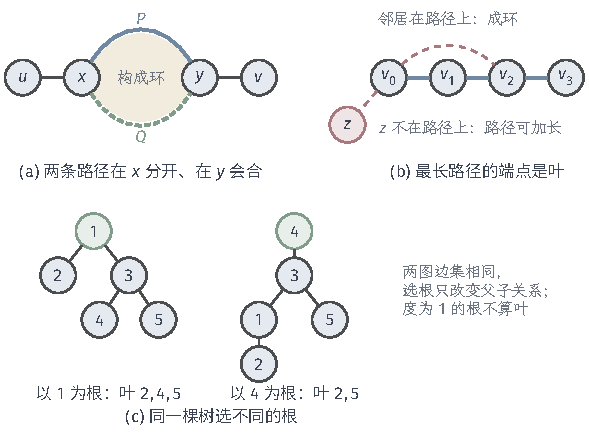
\includegraphics[width=99.688mm]{figures/01-basic-mathematics/04-graphs/tikz/c1-tree-properties/figure.pdf}
  \caption{树的性质的证明示意与选根。(a)两条不同的路径$P$（蓝色实线）与$Q$（绿色虚线）在$x$分开、在$y$第一次会合，二者之间的部分（黄色区域的边界）构成一个环。(b)若最长路径的端点$v_0$还有别的邻居，这个邻居不在路径上时可以把路径加长，在路径上时则形成环，两种情形都不可能。(c)同一棵树分别以$1$和$4$为根（绿色），边集不变，父子关系和叶的集合随根改变。}
  \label{fig:graph-conn-tree-properties}
\end{figure}

\paragraph{叶的存在}
数树的边数要用到度为$1$的顶点。无向图中度为$1$的顶点称为\term{叶}（leaf）。

\begin{lemma}[树有叶]
\label{lem:graph-conn-tree-leaves}
至少有两个顶点的树至少有两个叶。
\end{lemma}

\begin{proof}
树有限，路径只有有限条，取一条最长的路径$P=(v_0,\ldots,v_k)$。树连通且至少有两个顶点，所以有边，$k\geq1$。$v_1$是$v_0$的邻居。若$v_0$另有邻居$z\neq v_1$，分两种情形。若$z$不在$P$上，$(z,v_0,v_1,\ldots,v_k)$是一条更长的路径，与$P$最长矛盾；若$z=v_t$在$P$上，则$t\geq2$，$(v_0,v_1,\ldots,v_t,v_0)$是长度为$t+1\geq3$的环，与树无环矛盾。所以$d_{v_0}=1$。同理$d_{v_k}=1$，而$v_0\neq v_k$，树至少有两个叶。
\end{proof}

\paragraph{边数}
叶只与一个顶点相连，删掉它不会断开其余部分。这使我们能对顶点数归纳。

\begin{theorem}[树的边数]
\label{thm:graph-conn-tree-edges}
有$n$个顶点的树恰有$n-1$条边。
\end{theorem}

\begin{proof}
对$n$归纳。$n=1$时单点树没有边。设$n\geq2$，并设结论对$n-1$个顶点的树成立。由引理~\ref{lem:graph-conn-tree-leaves}，树$\mathcal T$有一个叶$v$，它只有一条邻边。考虑$\mathcal T-\{v\}$：它无环，因为删除顶点不会产生新环；它连通，因为$\mathcal T$中连接另外两个顶点的路径不会经过$v$——路径的中间顶点要有两条路径上的邻边，而$v$的度为$1$。所以$\mathcal T-\{v\}$是有$n-1$个顶点的树，由归纳假设有$n-2$条边。删除$v$只去掉一条边，$\mathcal T$有$n-1$条边。
\end{proof}

\paragraph{用边数判断树}
定理~\ref{thm:graph-conn-tree-edges}的逆命题需要加上连通的条件。先说明任何连通图都能用$n-1$条边连成一棵树，再比较边数。

设$\mathcal G$连通，任取一个顶点$r$，令已选顶点集$S=\{r\}$、已选边集$F=\varnothing$。只要$S\neq V$，就取一个$S$外的顶点$t$和一条从$r$到$t$的路径；路径从$S$内出发、在$S$外结束，其中必有一步从$S$内的顶点走到$S$外的顶点，把这一步的边加入$F$，把它的$S$外端点加入$S$。每一步恰好增加一个顶点和一条边，所以$n-1$步后$S=V$，$|F|=n-1$。

所得的$(V,F)$连通，因为每个新顶点都通过一条边连到先前已选的顶点上，归纳可知每个顶点都连到$r$。它也无环：若$F$中有环，取环上最后加入$S$的顶点$t$，它在环上的两个邻居都比它先加入。$F$中的每条边都在它的较晚端点加入时选出，并且连到一个更早的顶点；所以$t$与更早顶点之间的边只有$t$加入时选出的那一条，不可能同时连到环上两个更早的邻居，矛盾。因此$(V,F)$是一棵树。

\begin{theorem}[连通且$n-1$条边的图是树]
\label{thm:graph-conn-connected-tree-test}
设$\mathcal G$是有$n\geq1$个顶点的连通无向图。若$\mathcal G$恰有$n-1$条边，则$\mathcal G$是树。
\end{theorem}

\begin{proof}
按上面的构造从$\mathcal G$中选出$n-1$条边组成树$(V,F)$。$F\subseteq E$且$|F|=n-1=|E|$，所以$F=E$，$\mathcal G=(V,F)$本身就是树。
\end{proof}

连通的条件不能去掉。三角形加一个孤立顶点（图~\ref{fig:graph-conn-components}(a)）有$4$个顶点、$3$条边，恰好满足“$n-1$条边”，却既不连通又有环，不是树。只数边可能少看了连接，也可能把边浪费在环上。

\subsection{有根树}
\label{sec:graph-conn-rooted-trees}

在家谱、文件目录或分治计算中，树上的顶点有上下层次。路径唯一性使我们可以从任意一个顶点出发，把整棵树组织成这样的层次。

\paragraph{父节点、子节点与子树}
在树$\mathcal T$中选定一个顶点$r$作为根，得到\term{有根树}（rooted tree）。对每个$v\neq r$，从$r$到$v$有唯一的路径，路径上紧挨在$v$之前的顶点称为$v$的\term{父节点}（parent），$v$称为它的\term{子节点}（child）。根没有父节点，其余每个顶点恰有一个父节点。从$r$到$u$的路径经过$v$的那些顶点$u$（包括$v$本身）组成以$v$为根的\term{子树}（subtree）。在有根树中，没有子节点的顶点称为叶。

图~\ref{fig:graph-conn-tree-properties}(c)是同一棵树以两种方式选根。以$1$为根时，$3$的父节点是$1$，子节点是$4,5$，叶是$2,4,5$；以$4$为根时，$3$的父节点变成$4$，子节点变成$1,5$，叶是$2,5$。注意根$4$的度为$1$，在无向树中是叶，在以它为根的有根树中却有子节点、不算叶；两种“叶”的含义只在根上可能不同。

\paragraph{选根只附加组织方式}
两种选根下边集完全相同，选根没有增删任何边，只是规定了每条边上哪一端是父节点。父子关系由选根唯一确定，换一个根就会改变。若愿意，也可以把每条边定向为从父节点指向子节点，得到一张有向图，其中每个顶点的直接前驱就是父节点；但有根树的方向来自选根，而一般有向图的弧方向是原始数据的一部分，两者不应混同。第~\ref{sec:graph-tree-dp}节在有根树上自下而上计算时，正是利用“每个子树只通过它的根与外界相连”这一点。

\subsection{生成树与生成森林}
\label{sec:graph-conn-spanning-trees}

道路网中常要选出一部分道路，使所有城市仍然连通且没有多余的环，例如只维护最少的道路，或在网络中规定一套不会循环转发的线路。这就是在原图中保留全部顶点、只选部分边构成一棵树。

\begin{definition}[生成树与生成森林]
\label{def:graph-conn-spanning-tree}
设$\mathcal G=(V,E)$是无向图。若子图$(V,F)$，$F\subseteq E$，是一棵树，就称它为$\mathcal G$的\term{生成树}（spanning tree）。若$(V,F)$是森林，并且它的连通分量与$\mathcal G$的连通分量相同，就称它为$\mathcal G$的\term{生成森林}（spanning forest）。
\end{definition}

连通图一定有生成树，第~\ref{sec:graph-conn-tree-properties}小节逐个接入顶点的构造选出的$(V,F)$就是一棵。生成树要覆盖全部顶点，所以只有连通图才有生成树。对一般无向图，在每个连通分量上各取一棵生成树，合起来就是生成森林。

\paragraph{生成森林的边数}
设$\mathcal G$有$n$个顶点、$c$个连通分量，第$k$个分量有$n_k$个顶点，$n_1+\cdots+n_c=n$。由定理~\ref{thm:graph-conn-tree-edges}，第$k$个分量上的生成树有$n_k-1$条边，所以任何生成森林的边数都是
\begin{equation}
\sum_{k=1}^{c}(n_k-1)=n-c.
\label{eq:graph-conn-spanning-forest-edges}
\end{equation}
例如三角形加孤立顶点有$n=4$、$c=2$，生成森林有$2$条边：三角形中任选两条边，孤立顶点自成单点树。同一个计数也适用于任何森林：$n$个顶点、$c$个分量的森林恰有$n-c$条边。因此无环且有$n-1$条边的图只有一个分量，也是树。

\paragraph{生成树不唯一}
贯穿图\eqref{eq:graph-conn-running-graph}有$n=4$，它的每棵生成树都有$3$条边。从$5$条边中选$3$条共有$\binom53=10$种选法。若选出的$3$条边有环，环的长度只能是$3$，即恰好选中三角形$\{1,2,3\}$或$\{2,3,4\}$的三条边，这样的选法有$2$种。其余$8$种选法无环且有$n-1=3$条边，由上一段都是树。图~\ref{fig:graph-conn-spanning-trees}列出了这$8$棵生成树。

\begin{figure}[!htb]
  \centering
  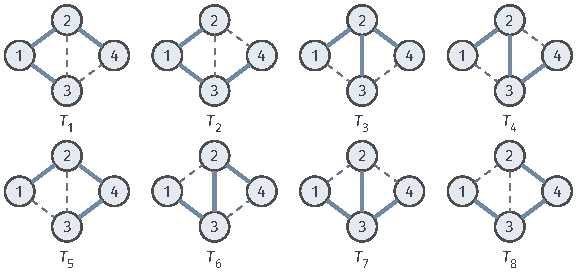
\includegraphics[width=97.652mm]{figures/01-basic-mathematics/04-graphs/tikz/c1-spanning-trees/figure.pdf}
  \caption{贯穿图的全部$8$棵生成树。蓝色粗线是树边，灰色虚线是被舍弃的原边。每棵生成树都有$3$条边并覆盖全部$4$个顶点；从$5$条边中选$3$条的$10$种选法里，只有恰好组成三角形$\{1,2,3\}$或$\{2,3,4\}$的两种不是树。}
  \label{fig:graph-conn-spanning-trees}
\end{figure}

\paragraph{抽取生成树会丢掉什么}
生成树保留了“全部顶点互相连通”，却舍弃了环所提供的替代路径，因此其他结构可能改变。以$T_2$（边$\{1,2\},\{1,3\},\{3,4\}$）为例：原图中$2,4$相邻，在$T_2$中却要经过$(2,1,3,4)$，路径长度从$1$变成$3$；原图删除任一顶点后仍连通，没有割点，而$T_2$中$1$和$3$都成了割点。所以在生成树上计算距离或分析脆弱性，结果一般不等于原图上的结果。

怎样用遍历高效地求出一棵生成树或生成森林，是第~\ref{chap:graph-traversal}章的内容；遍历得到的生成树只保证连通，不比较边权。当边带有建设成本时，从众多生成树中选出总成本最小的一棵，是第~\ref{sec:graph-minimum-spanning-tree}节研究的另一个问题。

\section{图的表示}
\label{sec:graph-representations}

前几节把图当作集合对$(V,E)$来推理。要让计算机处理一张图，还得决定怎样存储它。不同的算法反复执行的操作不同：有的逐条扫描所有边，有的反复列出一个顶点的全部邻居，有的要查询两个顶点之间是否有边，还有的要做矩阵运算。本节比较四种常用的表示，说明各自支持哪种访问、存储和访问代价怎样随顶点数$n$与边数$m$增长。代价用第~\ref{sec:comb-growth-scales}小节的记号$O(\cdot)$表示，例如“存储量为$O(n+m)$”指存储量不超过$n+m$的某个常数倍。图~\ref{fig:graph-conn-four-representations}把贯穿图的四种表示放在一起，供各小节对照。从矩阵出发构造图上的算子并研究其谱，集中在第~\ref{chap:graph-spectral}章。

\begin{figure}[!htb]
  \centering
  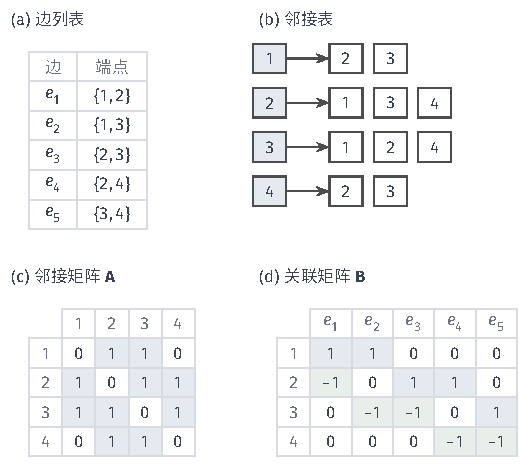
\includegraphics[width=89.524mm]{figures/01-basic-mathematics/04-graphs/tikz/c1-four-representations/figure.pdf}
  \caption{贯穿图的四种表示。(a)边列表逐条记录边的编号和端点；(b)邻接表为每个顶点（蓝色方框）列出邻居，每条无向边在两端各出现一次；(c)邻接矩阵按顶点次序记录每对顶点是否相邻，蓝色为$1$；(d)关联矩阵的每列对应一条边，按“小编号指向大编号”的记录方向，起点处为$1$（蓝色）、终点处为$-1$（绿色）。}
  \label{fig:graph-conn-four-representations}
\end{figure}

\subsection{边列表}
\label{sec:graph-conn-edge-list}

最直接的做法是把边一条条记下来。\term{边表}（edge list），也称边列表，为每条边保存一条记录：边的编号、两个端点，以及长度、容量等所需的属性。有向图的记录必须保存端点的次序，$(i,j)$与$(j,i)$是不同的弧。

图~\ref{fig:graph-conn-four-representations}(a)是贯穿图的边列表，$5$条无向边各占一条记录，记录中端点的先后没有意义。若扩展到有平行边的图，两条连接同一对顶点的边端点相同，只能靠编号区分，这时编号是记录中不可省略的部分。

\paragraph{访问方式与代价}
边列表除记录顶点集外只需$O(m)$的存储，适合需要逐条处理全部边的算法：例如按边权把所有边排序，或者在每一轮中把每条边都检查一遍。它的弱点是查询局部信息。要列出顶点$2$的邻居，或判断$\{1,4\}$是否为边，在没有额外索引时只能从头到尾扫描全部$m$条记录。第~\ref{sec:graph-minimum-spanning-tree}节按边权排序选边、第~\ref{sec:graph-shortest-paths}节逐轮检查每条边，用的都是这种访问方式。

\subsection{邻接表}
\label{sec:graph-conn-adjacency-list}

遍历一张图时，最频繁的操作是“列出当前顶点的全部邻居”。\term{邻接表}（adjacency list）为此而设计：给每个顶点保存一个列表，列出它的邻居，需要时连同对应边的属性一起保存。无向边$\{i,j\}$既出现在$i$的列表中，也出现在$j$的列表中；有向图的邻接表默认只保存出邻居，即$i$的列表是$N^+(i)$。

\paragraph{从边列表转换}
给$n$个顶点各建一个空列表，然后扫描边列表：遇到无向边$\{i,j\}$，就把$j$加入$i$的列表、把$i$加入$j$的列表；遇到弧$(i,j)$，只把$j$加入$i$的列表。转换用$O(n+m)$的时间。对贯穿图执行这一过程就得到图~\ref{fig:graph-conn-four-representations}(b)，顶点$2$的列表是$1,3,4$，长度恰好是度$d_2=3$。若算法还要沿弧反向查找，例如列出能一步到达$j$的全部顶点，就需要另建一份入邻居表，存储随之增加$O(m)$。

\paragraph{存储与访问代价}
邻接表有$n$个列表头；无向图的列表项共$\sum_i d_i=2m$个（式\eqref{eq:graph-conn-handshake}），有向图的出邻居表共$m$个。所以存储量为$O(n+m)$。列出顶点$i$的全部邻居只需读它自己的列表，时间与$d_i$成正比，不必触及与$i$无关的边；判断$\{i,j\}$是否为边则要在$i$的列表中查找，最坏需要$O(d_i)$时间。若一个算法对每个顶点都恰好列出一次邻居，总工作量就是$\sum_i(1+d_i)=n+2m$，即$O(n+m)$。第~\ref{chap:graph-traversal}章分析遍历的开销时，正是这样把实际访问次数累加起来。

\subsection{邻接矩阵}
\label{sec:graph-conn-adjacency-matrix}

查询“$i,j$是否相邻”时，邻接表要在列表里查找。若预先给每一对顶点留一个位置，这个查询就能一步完成，代价是更多的存储。

\paragraph{定义与方向约定}
固定顶点次序$1,\ldots,n$。无权图的\term{邻接矩阵}（adjacency matrix）$\bm A\in\mathbb R^{n\times n}$定义为
\[
a_{i,j}=
\begin{cases}
1, & \{i,j\}\in E\ \text{（有向图中为}\ (i,j)\in E\text{）},\\
0, & \text{其他情形}.
\end{cases}
\]
带权时把有边位置的$1$换成边权$w_{i,j}$，记作$\bm W$。有向图采用“行是起点、列是终点”的约定，第$i$行记录$i$的出邻居，第$j$列记录$j$的入邻居。无向图中$\{i,j\}$与$\{j,i\}$是同一条边，所以$\bm A$是对称矩阵；有向图的邻接矩阵一般不对称。贯穿图的邻接矩阵是
\begin{equation}
\bm A=
\begin{bmatrix}
0&1&1&0\\
1&0&1&1\\
1&1&0&1\\
0&1&1&0
\end{bmatrix},
\label{eq:graph-conn-running-adjacency}
\end{equation}
即图~\ref{fig:graph-conn-four-representations}(c)。第$i$行中$1$的个数就是度$d_i$，对角元全为$0$，对应没有自环。

\paragraph{零权边与结构掩码}
第~\ref{sec:graph-conn-weights}小节说过，零权边仍是边。在权矩阵$\bm W$中，零权边与无边的位置都存成$0$，单看$\bm W$无法区分图~\ref{fig:graph-conn-weight-semantics}(d)与(e)。允许零权边时，要另存一个结构掩码$\bm M\in\{0,1\}^{n\times n}$：有边处$m_{i,j}=1$，无边处为$0$。“是否相邻”查$\bm M$，“沿边累计多少”查$\bm W$；使用矩阵的算法应当说明它读的是哪一个。

\paragraph{稠密存储与稀疏存储}
把$n^2$个条目全部存下来称为稠密存储。它查询一对顶点是否相邻只需$O(1)$时间，但列出一个顶点的邻居要扫描整行，需要$O(n)$时间，即使该顶点只有一两个邻居。很多实际的图每个顶点只有少数邻居，$m$远小于$n^2$：例如一个道路网有$10^5$个路口，每个路口连着几条道路，边数只是几十万量级，而稠密邻接矩阵需要$10^{10}$个条目，绝大多数是$0$。稀疏存储只保存非零条目的位置和数值，存储量为$O(n+m)$，按行访问时与邻接表相当。因此说一个算法的代价时，必须同时说明图采用哪种存储：在邻接表上为$O(n+m)$的遍历，搬到稠密矩阵上逐行扫描就变成$O(n^2)$。

\paragraph{矩阵的幂计数行走}
把图写成矩阵，就能用第~\ref{sec:ls-matrix-operations}小节的矩阵乘法计算图的性质。按乘法定义，$(\bm A^2)_{i,j}=\sum_{\ell}a_{i,\ell}a_{\ell,j}$。乘积$a_{i,\ell}a_{\ell,j}$等于$1$，当且仅当$i$与$\ell$相邻并且$\ell$与$j$相邻，即$(i,\ell,j)$是一条长度为$2$的行走；否则乘积为$0$。所以对中间顶点$\ell$求和，数出的正是从$i$到$j$长度为$2$的行走条数。这一观察可以推广到任意长度。

\begin{theorem}[邻接矩阵的幂计数行走]
\label{thm:graph-conn-adjacency-powers}
设$\bm A$是无权图（无向或有向）的邻接矩阵，$k\geq0$为整数。则$(\bm A^k)_{i,j}$等于从$i$到$j$长度为$k$的行走条数。
\end{theorem}

\begin{proof}
对$k$归纳。$k=0$时$\bm A^0=\bm I$：长度为零的行走只有停在原地的$(i)$，所以从$i$到$i$恰有一条，$i\neq j$时没有，与单位矩阵一致。设结论对$k$成立。从$i$到$j$长度为$k+1$的行走$(i=v_0,\ldots,v_k,v_{k+1}=j)$可以按倒数第二个顶点$\ell=v_k$分类：它由一条从$i$到$\ell$长度为$k$的行走接上一步$\ell\to j$组成，而这一步存在当且仅当$a_{\ell,j}=1$。不同的$\ell$给出不同的类，每条行走恰好落入一类，所以
\[
\#\{\text{从}\ i\ \text{到}\ j\ \text{长度为}\ k+1\ \text{的行走}\}
=\sum_{\ell=1}^{n}(\bm A^k)_{i,\ell}\,a_{\ell,j}
=(\bm A^{k+1})_{i,j},
\]
其中第一个等号用了归纳假设，第二个等号是矩阵乘法的定义。
\end{proof}

对贯穿图直接计算，
\[
\bm A^2=
\begin{bmatrix}
2&1&1&2\\
1&3&2&1\\
1&2&3&1\\
2&1&1&2
\end{bmatrix}.
\]
图~\ref{fig:graph-conn-adjacency-square}说明$(\bm A^2)_{1,4}=a_{1,2}a_{2,4}+a_{1,3}a_{3,4}=2$，对应两条行走$(1,2,4)$与$(1,3,4)$。对角元$(\bm A^2)_{i,i}=d_i$，数的是从$i$出发走到一个邻居再立刻返回的闭行走，例如$(1,2,1)$与$(1,3,1)$；它们沿同一条边往返，并不是环。

\begin{figure}[!htb]
  \centering
  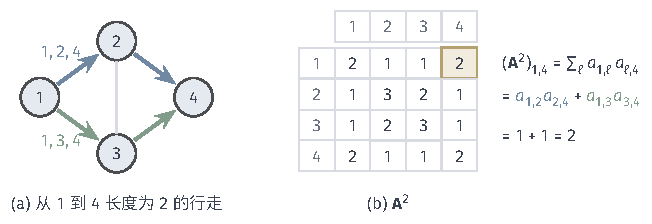
\includegraphics[width=110.352mm]{figures/01-basic-mathematics/04-graphs/tikz/c1-adjacency-square-walks/figure.pdf}
  \caption{邻接矩阵的平方计数长度为$2$的行走。(a)从$1$到$4$的两条行走$(1,2,4)$（蓝色）与$(1,3,4)$（绿色），中间顶点分别是$2$和$3$；(b)贯穿图的$\bm A^2$，黄色条目$(\bm A^2)_{1,4}=2$按中间顶点$\ell$求和，只有$\ell=2,3$的两项非零。}
  \label{fig:graph-conn-adjacency-square}
\end{figure}

这个计数包含重复顶点的行走，不能直接当作路径数或环数使用。例如可以算出$\bm A^3$的对角元依次为$2,4,4,2$，迹为$12$；长度为$3$的闭行走$(v_0,v_1,v_2,v_0)$中相邻两项都不相同（没有自环），于是三个顶点两两相邻，恰好组成一个三角形；而每个三角形可以从$3$个顶点出发、沿$2$个方向绕行，所以三角形个数为$12/6=2$，即$\{1,2,3\}$与$\{2,3,4\}$。更长的闭行走就会混入往返与重复绕行，不能这样简单换算。

带权时，同样的归纳说明$(\bm W^k)_{i,j}$等于所有从$i$到$j$长度为$k$的行走上边权乘积之和。它既不是行走条数，也不是路线长度之和：若边权表示长度，要求的是沿路线相加再取最小，这需要把矩阵乘法中的乘法换成加法、把求和换成取最小值，已经改变了运算规则。路线长度的最优化属于第~\ref{sec:graph-shortest-paths}节。

\subsection{关联矩阵}
\label{sec:graph-conn-incidence-matrix}

邻接矩阵以顶点对为单位，看不出“第几条边”。有些计算需要以边为单位，例如对每条边取出两个端点上的数值作比较。这就要一个行对应顶点、列对应边的矩阵。

\paragraph{定义与逐列核对}
把边编号为$e_1,\ldots,e_m$，并给每条无向边任选一个记录方向，例如把$e_k=\{i,j\}$记为从$i$到$j$。\term{关联矩阵}（incidence matrix）$\bm B\in\mathbb R^{n\times m}$的第$k$列在起点$i$处为$1$、在终点$j$处为$-1$，其余为$0$。有向图直接用弧的方向作为记录方向。

对贯穿图按图~\ref{fig:graph-conn-four-representations}(a)的编号，并统一取“小编号指向大编号”的记录方向，得到
\begin{equation}
\bm B=
\begin{bmatrix}
1&1&0&0&0\\
-1&0&1&1&0\\
0&-1&-1&0&1\\
0&0&0&-1&-1
\end{bmatrix},
\label{eq:graph-conn-running-incidence}
\end{equation}
即图~\ref{fig:graph-conn-four-representations}(d)。逐列读：第$1$列在第$1$行为$1$、第$2$行为$-1$，正是边$e_1=\{1,2\}$；第$5$列在第$3,4$行，正是$e_5=\{3,4\}$。每列恰有两个非零元，且和为$0$；第$i$行的非零元个数等于度$d_i$，例如第$2$行有三个。关联矩阵的每一列与边列表的一条记录一一对应，只是把端点写成了带符号的列向量。

\paragraph{记录方向的选择}
无向边的记录方向是任意选的。把第$k$条边的记录方向反过来，第$k$列整列变号，相当于把$\bm B$右乘一个对角元为$\pm1$的对角矩阵；图本身没有任何改变。所以对无向图，不同的记录方向给出同一张图的不同编码，后续计算若要反映图的性质，结果就不应依赖这一选择。有向图则不同：弧的方向是数据的一部分，反转它就得到另一张有向图。关联矩阵怎样计算每条边两端数值的差，以及它与拉普拉斯矩阵的关系，在第~\ref{sec:graph-vertex-edge-functions}节和第~\ref{sec:graph-laplacian}节展开。

\paragraph{四种表示的比较}
表~\ref{tab:graph-conn-representation-costs}汇总了本节讨论的代价。没有一种表示在所有操作上都最好：逐边处理用边列表，逐点列邻居用邻接表，频繁查询顶点对或做矩阵运算用邻接矩阵，以边为单位的线性计算用关联矩阵。实际程序常同时保存两种表示，额外的存储也应计入代价。

\begin{table}[!htb]
  \centering\small
  \begin{tabular}{@{}lccc@{}}
    \toprule
    表示 & 存储 & 列出$i$的邻居 & 查询$\{i,j\}$是否为边\\
    \midrule
    边列表 & $O(n+m)$ & $O(m)$ & $O(m)$\\
    邻接表 & $O(n+m)$ & $O(d_i)$ & $O(d_i)$\\
    稠密邻接矩阵 & $O(n^2)$ & $O(n)$ & $O(1)$\\
    稠密关联矩阵 & $O(nm)$ & $O(m+d_in)$ & $O(m)$\\
    \bottomrule
  \end{tabular}
  \caption{四种表示的存储与两种基本访问的时间代价，$n$为顶点数，$m$为边数，$d_i$为顶点$i$的度。边列表、邻接表不附加索引；稠密关联矩阵列出邻居时先扫描第$i$行找出$d_i$条邻边，再在每条边的列中找另一个端点。关联矩阵若改用按行、按列都可访问的稀疏存储，存储降为$O(n+m)$，列出邻居的代价与邻接表相当。}
  \label{tab:graph-conn-representation-costs}
\end{table}

\section{图同构}
\label{sec:graph-isomorphism}

顶点的名称只是为了区分顶点而取的。把贯穿图的顶点换一套编号，边集的写法会变，邻接矩阵的行列也会移动，连接结构本身却没有变。比较两张图时，需要一个标准来判断它们是否只差一套名称。本节先用保持邻接的一一对应定义同构，再用第~\ref{sec:prelim-common-matrices}小节的置换矩阵把重编号写成矩阵运算。怎样系统地比较两张图的结构，是第~\ref{sec:graph-wl-refinement}节的内容；这里先把要判定的目标说清楚。

\subsection{图同构的定义}
\label{sec:graph-conn-isomorphism-definition}

图~\ref{fig:graph-conn-isomorphism}(a)是贯穿图$\mathcal G$；(c)的$\mathcal G'$顶点集也是$\{1,2,3,4\}$，边集由$\{1,3\}$、$\{1,4\}$、$\{2,3\}$、$\{2,4\}$、$\{3,4\}$组成，画出来有两条边交叉，看上去与菱形不同。若按(b)的规则$\rho$把$\mathcal G$的顶点改名，$\mathcal G$的五条边依次变为
\[
\begin{gathered}
\{1,2\}\mapsto\{1,3\},\qquad
\{1,3\}\mapsto\{1,4\},\qquad
\{2,3\}\mapsto\{3,4\},\\
\{2,4\}\mapsto\{3,2\},\qquad
\{3,4\}\mapsto\{4,2\},
\end{gathered}
\]
恰好是$\mathcal G'$的全部边；唯一不相邻的一对$\{1,4\}$变为$\{1,2\}$，在$\mathcal G'$中也不相邻。两张图只差一套名称。

\begin{figure}[!htb]
  \centering
  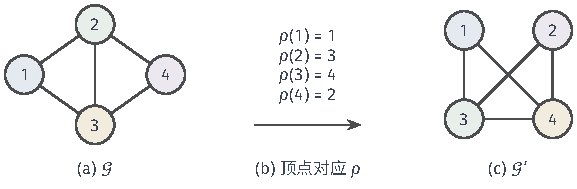
\includegraphics[width=97.688mm]{figures/01-basic-mathematics/04-graphs/tikz/c1-isomorphism-relabeling/figure.pdf}
  \caption{两张同构的图。(a)贯穿图$\mathcal G$；(c)画法与编号都不同的$\mathcal G'$；(b)顶点对应$\rho$。同色顶点互相对应：$\mathcal G$中顶点$i$与$\mathcal G'$中顶点$\rho(i)$颜色相同。逐条核对可见，$\mathcal G$中相邻的顶点对恰好对应$\mathcal G'$中相邻的顶点对。}
  \label{fig:graph-conn-isomorphism}
\end{figure}

\begin{definition}[图同构]
\label{def:graph-conn-isomorphism}
设$\mathcal G=(V,E)$与$\mathcal G'=(V',E')$是无向图。若存在双射$\rho:V\to V'$，使对任意$i,j\in V$都有
\[
\{i,j\}\in E\iff\{\rho(i),\rho(j)\}\in E',
\]
就称$\mathcal G$与$\mathcal G'$\term{同构}（isomorphic），称$\rho$为一个同构映射。
\end{definition}

定义中的双向条件不能减弱为单向。若只要求“$\mathcal G$的边映为$\mathcal G'$的边”，那么把边集为$\{1,2\},\{2,3\}$的路径按恒等映射放进三角形$\{1,2,3\}$也满足要求，但三角形多出了边$\{1,3\}$，两张图的边数不同。反方向的条件保证$\mathcal G'$中不出现$\mathcal G$里没有的连接，即保持不相邻关系。

\paragraph{有向图、加权图与带属性的图}
附加信息越多，同构要保持的东西越多。有向图的同构要求$(i,j)\in E\iff(\rho(i),\rho(j))\in E'$，即保持弧的方向；单向链$1\to2\to3$与$1\to2\leftarrow3$的底层无向图相同，作为有向图却不同构：后者的顶点$2$入度为$2$，前者每个顶点的入度至多为$1$，而有向图的同构映射保持入度。加权图还要求对应的边权相等，$w'_{\rho(i),\rho(j)}=w_{i,j}$；带属性的图则要由问题声明哪些属性必须保持，例如比较两个分子时原子种类必须一致，而原子的编号无关紧要。

\paragraph{用不变量排除同构}
同构映射保持一切由连接结构定义的量：顶点数、边数、每个顶点的度（$\rho$把$i$的邻居一一映为$\rho(i)$的邻居），因而还有全部顶点的度构成的多重集合，以及连通分量的个数、三角形的个数等。这些量称为图的不变量。只要有一个不变量不同，两张图就不同构。例如六个顶点排成一个环，与两个互不相连的三角形相比，顶点数、边数都是$6$，每个顶点的度都是$2$，但前者连通、后者有两个分量，所以不同构。

不变量相同却不足以断定同构。考虑两棵六个顶点的树，边集分别为
\[
\bigl\{\{1,2\},\{1,3\},\{1,4\},\{2,5\},\{3,6\}\bigr\}
\quad\text{与}\quad
\bigl\{\{1,2\},\{1,3\},\{1,4\},\{2,5\},\{5,6\}\bigr\}.
\]
二者都连通、没有三角形，度的多重集合都是$\{3,2,2,1,1,1\}$。但在前一棵树中，唯一的度为$3$的顶点$1$与两个度为$2$的顶点$2,3$相邻；在后一棵树中，顶点$1$只与一个度为$2$的顶点$2$相邻，另一个度为$2$的顶点$5$不是它的邻居。同构映射必须把度为$3$的顶点映到度为$3$的顶点，并保持它的邻居及邻居的度，所以两棵树不同构。这个例子提示，比较“邻居的度”能区分只看度区分不了的图；第~\ref{sec:graph-wl-refinement}节的顶点标记细化正是把这一想法反复执行。逐个尝试全部$n!$个双射虽然总能判定，但随$n$增长得太快，不能作为实用的方法。

\subsection{重编号与置换表示}
\label{sec:graph-conn-relabeling}

当两张图的顶点集都是$\{1,\ldots,n\}$时，同构映射$\rho$就是一个重编号：把顶点$i$改称为$\rho(i)$。重编号以后，邻接矩阵的行和列都要按同样的方式重新排列。第三部分的置换矩阵恰好执行这种重排。

\paragraph{置换共轭}
按第~\ref{sec:prelim-common-matrices}小节，取置换矩阵$\bm P=\begin{bmatrix}\bm e_{\rho(1)}&\cdots&\bm e_{\rho(n)}\end{bmatrix}$，它满足$\bm P\bm e_i=\bm e_{\rho(i)}$。由第~\ref{sec:ls-matrix-operations}小节置换矩阵的乘法规则，左乘$\bm P$把第$i$行移到第$\rho(i)$行；右乘$\bm P^{\top}$相当于对转置后的矩阵左乘$\bm P$，把第$j$列移到第$\rho(j)$列。两者合起来，
\begin{equation}
\bm A'=\bm P\bm A\bm P^{\top},\qquad
a'_{\rho(i),\rho(j)}=a_{i,j}.
\label{eq:graph-conn-relabel}
\end{equation}
第二式说明，原来记录“$i,j$是否相邻”的条目被搬到了新编号$\rho(i),\rho(j)$的位置。因此，$\rho$是$\mathcal G$到$\mathcal G'$的同构映射，当且仅当$\mathcal G'$的邻接矩阵等于$\bm P\bm A\bm P^{\top}$。

\paragraph{核对贯穿图的例子}
对图~\ref{fig:graph-conn-isomorphism}的$\rho$，$\bm P$的各列依次为$\bm e_1,\bm e_3,\bm e_4,\bm e_2$。由式\eqref{eq:graph-conn-running-adjacency}计算得
\[
\bm P=
\begin{bmatrix}
1&0&0&0\\
0&0&0&1\\
0&1&0&0\\
0&0&1&0
\end{bmatrix},\qquad
\bm P\bm A\bm P^{\top}=
\begin{bmatrix}
0&0&1&1\\
0&0&1&1\\
1&1&0&1\\
1&1&1&0
\end{bmatrix}.
\]
右边矩阵的第$1$行在第$3,4$列为$1$，即$N'(1)=\{3,4\}$；第$4$行在第$1,2,3$列为$1$，即$N'(4)=\{1,2,3\}$；各行都与$\mathcal G'$的边集一致。逐个位置看也是如此，例如$a'_{3,2}=a'_{\rho(2),\rho(4)}=a_{2,4}=1$。加权图把$\bm A$换成$\bm W$，同样要求$\bm W'=\bm P\bm W\bm P^{\top}$；允许零权边时，还要同时检验结构掩码$\bm M'=\bm P\bm M\bm P^{\top}$，因为两个顶点之间无边与有一条零权边，权矩阵都是零矩阵。

\paragraph{置换不同于一般换基}
置换矩阵满足$\bm P^{\top}\bm P=\bm I$，所以$\bm P^{\top}=\bm P^{-1}$，式\eqref{eq:graph-conn-relabel}是第~\ref{sec:ls-similarity}小节意义下的相似变换。但反过来，一般的相似变换$\bm S\bm A\bm S^{-1}$不能都解释为重编号。例如对两个顶点一条边的图，$\bm A=\left[\begin{smallmatrix}0&1\\1&0\end{smallmatrix}\right]$，取$\bm S=\left[\begin{smallmatrix}1&1\\0&1\end{smallmatrix}\right]$，得到
\[
\bm S\bm A\bm S^{-1}
=\begin{bmatrix}1&1\\0&1\end{bmatrix}
\begin{bmatrix}0&1\\1&0\end{bmatrix}
\begin{bmatrix}1&-1\\0&1\end{bmatrix}
=\begin{bmatrix}1&0\\1&-1\end{bmatrix},
\]
它不对称，有非零对角元和负条目，已经不是任何简单无向图的邻接矩阵。一般换基会把不同顶点的坐标混合起来，而重编号只搬动位置、不混合数值。相似变换保持特征值，所以同构的图有相同的邻接矩阵特征值；这一事实的用途和局限在第~\ref{chap:graph-spectral}章讨论，这里只确定重编号的精确含义。

\section{本章小结}
\label{sec:graph-objects-summary}

本章围绕三个问题建立了图的基本语言：连接是什么，沿连接能到哪里，结构怎样记录和比较。图$\mathcal G=(V,E)$只记录有限个对象之间的直接连接，与纸上的画法无关。方向、边权和属性各自附加一类信息：方向决定哪些顶点序列可以通行，边权的含义由问题决定，长度相加、容量限制通过量、相似度鼓励两端接近；零权边仍是边，“能否到达”查边集，“累计多少”查边权。子图与诱导子图区分了“任意保留一部分边”和“保留选定顶点之间的全部边”。

沿连接能到哪里，由行走和路径回答。行走允许重复，便于拼接与计数；路径不重复顶点，对应实际路线；任何行走中都含有一条同端点的路径，所以判断可达时两者等价。无向图中可达关系是等价关系，把顶点集唯一地划分为连通分量；有向图中可达不对称，需要区分要求双向到达的强连通与忽略方向的弱连通，前者蕴含后者而反之不然。分隔集、割点和桥刻画了删除顶点或边对连接的影响，判断的依据始终是有没有替代路径：一条边是桥，当且仅当它不在任何环上。树是连通而无环的图，等价于任意两点之间路径唯一；$n$个顶点的树恰有$n-1$条边，连通且有$n-1$条边的图是树，而$n$个顶点、$c$个分量的生成森林恰有$n-c$条边。

同一张图可以用边列表、邻接表、邻接矩阵和关联矩阵记录，四者保存的连接相同，支持的访问和代价不同；邻接矩阵还把图的组合问题与矩阵运算联系起来，$\bm A^k$的条目计数长度为$k$的行走，但其中包含重复顶点。同构用保持邻接与不相邻的双射刻画“只差一套名称”，在矩阵上表现为置换共轭$\bm A'=\bm P\bm A\bm P^{\top}$；度、分量数等不变量可以排除同构，却不足以确认同构。拿到一张图时，可以用这些表示和不变量核对：所关心的结构是否被保留，附加的数值和方向是否交代清楚。

本章定义了连通分量、强连通分量、生成树、有向无环图上的依赖和同构，却还没有给出高效求出它们的方法。第~\ref{chap:graph-traversal}章在邻接表上用广度优先和深度优先遍历实际计算这些对象，用拓扑排序安排有向无环图的次序，并用顶点标记细化比较图的结构；那里的算法输出，仍要按本章的定义与条件检验。

